\documentclass[11pt, a4j]{jreport}

\usepackage{comment}
\usepackage{float}
\usepackage{color}
\usepackage{multicol}
\usepackage[dvipdfmx]{pict2e}
\usepackage{wrapfig}
\usepackage{graphicx}
\usepackage{bm}
\usepackage{url}
\usepackage{underscore}
\usepackage{colortbl}
\usepackage{tabularx}
\usepackage{fancyhdr}
\usepackage{ulem}
\usepackage{cite}
\usepackage{amsmath, amssymb, amsfonts}
\usepackage{algorithmic}
\usepackage{textcomp}
\usepackage{xcolor}
\usepackage[ipaex]{pxchfon}

\usepackage[top=30truemm, bottom=30truemm, left=25truemm, right=25truemm]{
    geometry
}

\begin{document}
    \thispagestyle{empty}
    \begin{center}
        \vspace{20mm}
        {\Large\noindent 2024年度 卒業(学士)論文}\\
        \vspace{40mm}
        {\huge\noindent\textbf{SNSにおける世論形成と紛争に関するReddit投稿分析}}\\
        \medskip
        {\huge\noindent\textbf{ーイスラエルによるレバノン侵攻を例にー}}\\
        \vspace{\baselineskip}
        \vspace{40mm}

        {\Large\noindent 2025年1月31日\\ \vspace{\baselineskip} 指導教員 崎田智子 \\ \vspace{\baselineskip} 同志社大学\\ グローバル地域文化学部グローバル地域文化学科アジア・太平洋コース \\ \vspace{\baselineskip} 1122192047 種村尚大\\ }
        \vspace{40mm}
    \end{center}

    \thispagestyle{empty}
    \clearpage

    %=====================================================================================
    \renewcommand{\abstractname}{要旨}

    \begin{abstract}
        研究の要旨。なんやかんやなんやかんやなんやかんやなんやかんやなんやかんやなんやかんやなんやかんやなんやかんやなんやかんやなんやかんやなんやかんやなんやかんやなんやかんやなんやかんやなんやかんやなんやかんやなんやかんやなんやかんやなんやかんやなんやかんや
    \end{abstract}

    %=====================================================================================

    % 目次の表示
    \tableofcontents

    %=====================================================================================
    \pagestyle{fancy}
    \lhead{\rightmark}
    \renewcommand{\chaptermark}[1]{\markboth{第\ \normalfont\thechapter\ 章~~#1}{}}
    %=====================================================================================

    \chapter{はじめに} %章

    \section{研究背景}

    21世紀における紛争の様相は、従来の軍事的な衝突に加え、情報空間における戦いの重要性が増している。特に、ソーシャルネットワーキングサービス(SNS)は、紛争に関する情報発信や議論の場として機能し、世論形成に強い影響を与えている。これらのプラットフォームは、リアルタイムでの情報共有、国際的な議論の可視化、多様な声の拡散を可能にしている。

    中でもRedditは、特異な構造と利用者特性を持つSNSとして注目されている。Redditは2005年に設立され、\textbf{2024年時点で月間アクティブユーザー数が約5億人に達している}(Statista, 2024)。その利用者層は主に北米とヨーロッパに集中しており、ユーザーの約50\%が18~34歳と比較的若い世代に偏っている。また、性別比率では男性が約60\%を占めるが、女性ユーザーも年々増加傾向にある(Reddit Demographics Report, 2024)。さらに、Redditのユーザーは教育水準が高く、大学卒業者が多いことも特徴の一つである。

    このプラットフォームの最大の特徴は、匿名性と分散型のコミュニティ構造にある。Redditは、\textbf{サブレディットと呼ばれる膨大な数の専門的なコミュニティで構成されており、それぞれが特定のトピックや興味に基づいて議論を展開する}。投稿やコメントは、ユーザーからの評価(アップボートまたはダウンボート)によってランキングされるため、コミュニティ全体の関心や優先順位が自然に反映される仕組みが採用されている。この構造は、特定の話題について多様な視点を集約し、リアルタイムで議論を活発化させる基盤を提供している。

    \textbf{2024年10月1日にイスラエルが実施したレバノン侵攻}は、国際社会における注目を集め、地域的な緊張を一層高める結果となった。この侵攻は、南レバノンを拠点とする武装組織ヒズボラによる攻撃への報復として行われたが、同時に人道危機を引き起こし、多くの民間人が犠牲となった。国連や人権団体は、即時停戦を呼びかける一方で、戦闘行為によるインフラの破壊と大規模な避難民の発生について深い懸念を表明した。

    このような状況の中、\textbf{SNS上の議論は急激に活発化}し、Redditでも紛争関連の投稿やコメントが急増した。特に、\textit{r/worldnews, r/politics, r/MiddleEast}などのサブレディットでは、侵攻に関する情報や意見交換が爆発的に広がり、国際社会の反応や一般ユーザーの感情がリアルタイムで可視化された。これらのプラットフォームは、紛争に関連する多様な視点を集約するだけでなく、特定の意見やナラティブがどのように形成され拡散するかを観察する上で極めて重要な役割を果たした。

    本研究では、このReddit上で観察される投稿数や感情の変化、議論のトピックの移り変わりを分析し、現代の紛争がデジタル空間でどのように議論されるのかを探る。

    \section{研究目的}
    本研究の目的は、2024年10月1日のイスラエルによるレバノン侵攻がReddit上の議論やユーザーの反応にどのような影響を与えたかを明らかにすることである。本研究は以下の3つの観点に焦点を当てる: 

    \begin{enumerate}
        \item 投稿数の変動: 紛争の発生が投稿数にどのような変化をもたらしたかを分析し、議論の活性化や関心の高まりを評価する。
        \item 感情的傾向の変化: 感情分析を用いて、紛争に対するユーザーの反応がどのように変化したかを明らかにする。
        \item トピックの変遷: 動的トピックモデリング(DTM)を活用し、議論が紛争直後の急性期からその後の段階にかけてどのように展開したかを時系列で追跡する。
    \end{enumerate}

    本研究は、SNSが国際紛争に与える影響を総合的に理解することを目指し、データ駆動型の分析手法を駆使して、以下の独自性を持つ知見を提供する: 

    \begin{enumerate}
        \item Redditという匿名性と分散型構造を持つプラットフォームの特性に着目し、これが国際紛争の議論に与える影響を詳細に分析する。
        \item 投稿数や感情スコアの分析に加え、トピックモデリングを用いることで、SNS上の議論がどのようにテーマを移行させていくかを具体的に明らかにする。
        \item サブサンプリングや差分の差分(DID)分析を活用し、介入(紛争発生)が議論の量的および質的側面に与える影響を因果的に評価する。
    \end{enumerate}

    \section{本論文の仮説}
    本研究では、以下の仮説を検証する: 
    \begin{enumerate}
        \item \textbf{投稿数の増減}: イスラエルによるレバノン侵攻は、紛争関連サブレディットにおける投稿数を急増させる一方で、対照群では投稿数の変化が限定的である。
        \item \textbf{投稿内容の過激化}: 紛争直後、投稿内容はネガティブかつ感情的な傾向を示し、センチメントスコアが低下する。
        \item \textbf{トピックの変遷}: 紛争に関する議論は、発生直後には戦闘や人道危機に集中し、時間の経過とともに国際支援や解決策の模索へと焦点が移る。
    \end{enumerate}

    \section{本論文の構成}
    本論文は以下の構成をとる: 
    \begin{itemize}
        \item 第2章: SNSにおける世論形成と国際紛争に関する先行研究のレビューを行い、Redditの特性について議論する。
        \item 第3章: データ収集および分析手法を説明し、投稿数、感情スコア、トピックの変化を調査するための具体的な方法論を提示する。
        \item 第4章: 分析結果を提示し、紛争がReddit上の議論に与える影響を示す。
        \item 第5章: 結果を解釈し、SNSが国際紛争における世論形成や情報拡散に果たす役割について考察する。
        \item 第6章: 本研究の結論をまとめ、今後の課題と研究の展望を示す。
    \end{itemize}

    本研究は、Redditという特異なプラットフォームにおける議論のダイナミクスを解明することで、デジタル時代の国際紛争におけるSNSの役割を理解するための新たな知見を提供することを目指している。この研究は、政策立案者や国際機関がデジタル空間を活用する際の参考となり得る重要な示唆を含んでいる。

    \chapter{SNSにおける世論形成と国際紛争に関する先行研究}

    \section{SNSと世論形成}
    ソーシャルネットワーキングサービス(SNS)は、21世紀において世論形成の重要なツールとなり、従来のマスメディアを補完する役割を果たしている。特に、情報が瞬時に広範囲に拡散され、多様な意見が可視化される点で、SNSは「集団行動を促進するツール」として位置づけられている(Shirky, 2011)。例えば、2010年代の「アラブの春」では、TwitterやFacebookを通じて市民がプロテストの呼びかけや情報共有を行い、社会運動の大規模化を支えたことが報告されている(Howard & Hussain, 2013)。このように、SNSは社会的・政治的な動員における迅速性と規模の拡大に寄与している。

    一方で、SNSにおける情報流通には限界も指摘されている。Sunstein(2001)やPariser(2011)は、エコーチェンバー現象やフィルターバブルが、ユーザーを特定の情報に偏らせるリスクを指摘している。たとえば、Facebookのアルゴリズムによるフィードの最適化が、政治的分断を助長する可能性があることが示されている。これらの現象は、SNSが多様な意見の交換を促進する一方で、逆に対話の閉鎖性を生む可能性があることを示唆している。

    さらに、SNSが選挙や緊急事態において果たす役割も注目されている。たとえば、2016年のアメリカ大統領選挙では、Twitterを通じての情報戦が候補者のイメージ形成に影響を与えたことが明らかにされている(Allcott & Gentzkow, 2017)。このように、SNSの利用は単なる情報共有を超え、世論形成における戦略的な要素としても機能している。

    \section{国際紛争におけるSNSの役割}
    SNSは国際紛争において、単なる情報共有の場を超え、プロパガンダや情報操作の場としても機能している。HowardとHussain(2013)は、アラブの春におけるSNSの役割について、情報の共有と抗議活動の組織化を促進する手段としての重要性を指摘している。また、Zeitzoff(2017)の研究では、イスラエルとハマスの紛争におけるTwitterの使用が、紛争当事者のソフトパワー的な戦略に寄与していることが示されている。たとえば、戦闘の進行状況をリアルタイムで伝えることで、国際的な支持を獲得する動きが観察されている。

    さらに、SNSは国際的な議論を加速させるツールとしても機能している。イスラエルとパレスチナの紛争では、世界中のユーザーがSNSを通じて意見を発信し、国際世論が紛争当事者への外交的プレッシャーとして作用するケースが見られる。これにより、SNSは紛争解決や国際支援のプロセスに間接的な影響を及ぼしている。

    BennettとSegerberg(2012)は、SNSが「ネットワーク化された個人的行動」を促進し、従来の組織化された抗議活動よりも分散的で迅速な動員を可能にすると述べている。この視点は、SNSが国際紛争の文脈において、情報共有だけでなく、個人の行動を直接的に動員する力を持つことを示唆している。

    \section{Redditの特異性}
    Redditは他のSNSと比較して匿名性が高く、ユーザーが特定のトピックに関心を持つコミュニティ(サブレディット)に参加することで、多様な意見交換が可能となるプラットフォームである。Massanari(2015)は、Redditの匿名性と分散型構造が、多様な視点を反映した議論を促進すると指摘している。また、「アップボート」「ダウンボート」の評価システムは、特定の意見が可視化される一方で、少数派の意見も一定の支持を得て拡散される可能性を持つ。

    特に、国際紛争に関する議論では、サブレディットごとに異なる視点が展開されることが多い。たとえば、「r/worldnews」ではグローバルな視点からの議論が行われる一方、「r/Israel」や「r/palestine」では地域特有の視点が強調される。GaffneyとMatias(2018)の研究によれば、Redditのコメントシステムは階層的な議論構造を生み出し、紛争の複雑な側面に関する多層的な議論を可能にしている。この特徴は、他のSNSでは観察されにくいReddit特有の性質といえる。

    さらに、Mills(2018)は、Redditのサブレディットが「想像の共同体」として機能する点を指摘しており、特定のイデオロギーや価値観を共有するユーザー間の結束を強化する傾向がある。この点は、Redditが紛争に関する議論においてどのように偏りを生じさせる可能性があるかを示唆している。

    \section{先行研究との関係}
    これまでの先行研究は、SNSが国際紛争や政治的動員に与える影響について、SNS全般の役割や、主にTwitterやFacebookといったプラットフォームの影響を分析してきた。たとえば、Shirky(2011)やHowardとHussain(2013)は、SNSがプロテスタントや社会運動の組織化を支援し、情報拡散を迅速化するツールとしての役割を強調している。また、Zeitzoff(2017)はTwitterを用いて、紛争当事者が戦略的なコミュニケーションを通じて国際的な支持を獲得する手段としてSNSを活用していることを示している。しかし、これらの研究は、特定のプラットフォームの独自性や、ユーザー間の議論ダイナミクスの詳細には踏み込んでおらず、SNSが個々のユーザーやコミュニティの世論形成にどのように作用するかについては限定的である。

    本研究は、これらの先行研究に対して以下の3つの点で独自性を持ち、学術的意義を提供する。

    \subsection*{1. Redditという未開拓プラットフォームへの着目}
    既存の研究の多くがTwitterやFacebookといった既成のSNSに焦点を当てている中で、本研究はRedditという匿名性が高く、分散型構造を持つプラットフォームを対象としている。Redditの特異性は、サブレディットというコミュニティ構造と、ユーザーがコンテンツを評価する投票システムにある。この特徴は、議論が多様な視点を含む形で展開される可能性を高める一方で、議論の偏りや極化を生むリスクも持つ。Massanari(2015)が示すように、Redditの評価システムは、少数意見や論争的な意見の可視性を保証する仕組みとして機能しており、これが世論形成に与える影響は他のSNSとは一線を画す。

    特に、本研究は、イスラエル・レバノン紛争という具体的な国際事件を題材に、Reddit上での議論のダイナミクスを分析することで、このプラットフォームが国際紛争に関連する世論形成や情報拡散に与える独自の影響を明らかにする。

    \subsection*{2. データ駆動型アプローチの統合}
    従来のSNS研究では、投稿数の変化や感情分析を用いた傾向の把握が主流であった。本研究ではこれらの手法に加え、動的トピックモデリング(DTM)を用いた議論のテーマの変遷分析を組み合わせることで、議論の量的変化だけでなく、その質的側面を時系列的に明らかにすることを試みている。

    具体的には、投稿数の急増や感情スコアの変化を検出するだけでなく、DTMを活用して、議論が「戦闘」「人道危機」「国際支援」などのトピックにどのように分布し、時間の経過とともにどのように移行していくかを分析した。この手法により、投稿者の関心がどの時点で特定のテーマに集中し、その後どのように新たなトピックへと推移していくかを詳細に把握することが可能となる。

    特に、紛争直後における投稿数や感情の急激な変化が、どのようなテーマと関連しているのかを検討することで、SNS上の議論形成のダイナミクスをより深く理解するための基盤を提供する。本研究のように量的データ(投稿数や感情スコア)と、トピックという質的側面を統合的に分析するアプローチは、SNS研究における新たな視点を提供するとともに、議論の全体像をより包括的に捉えることに寄与する。    

    \subsection*{3. 国際紛争とオンライン世論の関係性への新たな知見}
    既存研究では、SNSが国際紛争において果たす役割が、情報拡散やプロテスタントの動員といった「直接的な効果」に焦点を当てることが多かった。一方で、本研究は、Reddit上の議論が紛争当事者への国際的な支持や批判を形成するだけでなく、SNS利用者同士の議論の焦点やトーンがどのように変化し、SNS全体の議論空間に影響を与えるかを検証している。具体的には、サブレディット間での視点の違いや、特定のテーマに対する議論の偏りが、紛争の認識や世論形成に与える影響を多角的に分析している。

    また、Redditが持つ匿名性や分散型構造の特性が、議論の質や偏りにどのように影響するかについても考察することで、従来のSNS研究では見落とされてきた議論の「質的側面」に光を当てている。この点で、本研究は単なる議論の量的変化にとどまらず、その内容や構造の変化を深く掘り下げている。

    \subsection*{4. SNS研究への学術的貢献と実践的意義}
    本研究は、Redditという未開拓のプラットフォームを対象とすることで、SNS研究に新たな学術的貢献を提供している。また、紛争や国際問題における世論形成のプロセスを明らかにすることは、政策立案者や国際機関にとって、SNSを活用した情報戦略の策定やデジタルディプロマシーの構築に向けた実践的な示唆を提供する。

    \chapter{データ収集・分析手法}
    本章では、Redditにおける投稿データを対象としたデータ収集および分析手法について詳述する。本研究では、信頼性と精度を確保しつつ、大規模な投稿データを効率的に取得するために適切なデータ収集アプローチを採用した。さらに、収集したデータを用いて、投稿数の変化、感情スコアの推移、および議論のトピックの変遷を分析するための方法論を提示する。これにより、データ駆動型の手法が本研究の目的を達成する上でなぜ有効であるかを論じる。

    \section{データ収集の方法}
    \subsection{PRAWおよびPushshift APIを用いたデータ収集}
    Redditのデータ収集には、PRAW (Python Reddit API Wrapper) を主に使用し、大規模かつ効率的なデータ取得を実現した。

    収集対象期間は、イスラエルによるレバノン侵攻(2024年10月1日)の影響を分析するため、2024年7月26日から2024年10月26日までの約3ヶ月間とした。この期間設定により、紛争勃発前の基準値、直後の急激な反応、そしてその後の議論の推移までを包括的にカバーできる。

    対象となるサブレディットは、イスラエル・パレスチナ問題に関連する議論が活発な「r/Israel」「r/Palestine」「r/IsraelPalestine」の3つに加え、対照群として、紛争と無関係な一般的なサブレディット「r/ps4homebrew」「r/Exercise」「r/voyageons」も収集した。これにより、紛争関連サブレディットにおける変化を対照的に比較する枠組みを構築した。

    データとしては各サブレディットにおけるsubmissionとそれに付随してコメントも取得対象とした。

    \section{投稿数の変化と差分の差分(DID)分析}
    投稿数の変化を分析するため、Pythonのmatplotlibおよびpandasライブラリを用いて時系列データを可視化した。データは1日単位で集計し、紛争勃発日(2024年10月1日)を基準として、紛争前後での投稿数の変動を比較した。

    さらに、紛争の影響を定量的に評価するため、差分の差分(Difference-in-Differences, DID)分析を実施した。DIDは観察データに基づき介入(今回の場合は紛争勃発)が結果に与える因果的な影響を推定する手法であり、紛争関連サブレディットと対照群サブレディットの間での投稿数の変化を比較することで、介入の純粋な効果を明らかにすることが可能である。

    \subsection*{サブサンプリングによるデータ調整}
    分析対象となるデータでは、処置群(紛争関連サブレディット)の投稿数が対照群(非紛争関連サブレディット)と比較して大幅に多いことが確認された。このデータの不均衡は、DID分析における結果の偏りや推定値の信頼性低下を招く可能性があるため、以下の手順でサブサンプリングを行った:

    \begin{enumerate}
        \item 対照群サブレディットの日次投稿数の平均を基準とし、処置群からランダムに同数の投稿を抽出。
        \item サブサンプリングは分析結果の安定性を確保するため、複数回(100回)繰り返し実施し、平均値を算出。
        \item サブサンプリングによるデータ調整後、DIDモデルを適用。
    \end{enumerate}

    このプロセスにより、処置群と対照群のデータ数の差を緩和し、DID分析における比較の公平性と信頼性を向上させた。この処理は後ほど説明する「感情分析とVADERスコアの時系列変化」でも同様に実施されている。

    \textbf{DIDを用いる必要性}
    DID分析を採用した理由は以下の通りである:
    \begin{enumerate}
        \item 介入の因果的影響を識別するため: 紛争勃発による投稿数の変化を単に観察するだけでは、紛争以外の要因(季節的な投稿数の変動、一般的なトレンドなど)が結果に影響を与えている可能性を排除できない。DIDは、紛争関連サブレディット(処置群)と、紛争と無関係なサブレディット(対照群)を比較することで、これらの外的要因を統制し、紛争の影響そのものを識別できる。
        \item 差分の差分に基づく純粋な影響推定: DIDは、以下のステップで介入効果を分離する:
            \begin{enumerate}
                \item 介入前後で処置群(紛争関連サブレディット)の投稿数変化を計算。
                \item 介入前後で対照群(非紛争関連サブレディット)の投稿数変化を計算。
                \item 処置群と対照群の変化量を比較(差分の差分)することで、介入の純粋な影響を推定。
            \end{enumerate}
            これにより、紛争がなかった場合の投稿数変化(対照群の変化を基に推定)をコントロールしつつ、紛争の影響を明確にすることができる。
        \item 観察データでの実践的有用性: DIDはランダム化実験が実施できない場合においても、因果推論を行うために広く用いられる手法である。今回のケースでは、紛争が自然発生的な事象であり、介入のタイミングを研究者が制御できないため、DIDは適切な分析手法といえる。
    \end{enumerate}
    \textbf{DIDモデルの仕様}
    DID分析では、以下の回帰式を使用した:

    \begin{equation}
        Y_{it} = \beta_{0} + \beta_{1}*Treatment_{i} + \beta_{2}*Post_{t} + \beta_{3}*(Treatment_{i} * Post_{t}) + \epsilon_{it}
    \end{equation}

    ここで、
    \begin{itemize}
        \item $Y_{it}$:日次投稿数(サブレディット$i$の時点$t$における投稿数)
        \item $Treatment_{i}$:紛争関連サブレディットであるか否か(1=処置群、0=対照群)
        \item $Post_{t}$:紛争勃発後の期間であるか否か(1=紛争後、0=紛争前)
        \item $(Treatment_{i} * Post_{t})$:処置群で紛争後の期間を示す相互作用項
        \item $\beta_{3}$:紛争の影響を表す推定値
    \end{itemize}

    \textbf{DIDの意義と期待される結果}
    DID分析の結果、$\beta_{3}$の推定値が正で有意であれば、紛争が紛争関連サブレディットの投稿数を有意に増加させたことを意味する。これにより、紛争がReddit上の議論活性化に与える直接的な影響を実証的に評価することが可能となる。

    また、対照群サブレディットを使用することで、紛争以外の要因(例:一般的な投稿数の増減、システム的な変化など)が分析結果に与える影響を排除し、結果の信頼性を高めている点が本研究の強みである。

    \section{感情分析とVADERスコアの時系列変化}

    \subsection*{VADERの仕組みとその意義}
    感情分析には、VADER(Valence Aware Dictionary and sEntiment Reasoner)を使用した。VADERは、ソーシャルメディアのような非構造化テキストに適した辞書ベースの感情分析ツールであり、短文、スラング、絵文字、強調表現(例:「!!!」「VERY」)などを含む多様な文脈を効果的に処理できるよう設計されている。

    VADERのアルゴリズムは、辞書に基づくアプローチを採用しており、単語やフレーズに事前に割り当てられた感情スコア(ポジティブ、ネガティブ、中立)を元に、文章全体の感情スコアを計算する。この辞書は、人間の評価者がラベル付けを行ったデータセットに基づいて構築されており、特にソーシャルメディアやニュースの文脈での利用を想定して作成されている。

    VADERが広く利用される理由は以下の通りである:
    \begin{itemize}
        \item ソーシャルメディア特有のスラングや絵文字、文脈的な意味を考慮できる。
        \item ポジティブ、ネガティブ、ニュートラルのスコアだけでなく、総合的な「コンパウンドスコア」を提供し、文全体の感情を包括的に評価可能。
        \item Pythonライブラリに統合されており、高速かつ簡便な処理が可能。
    \end{itemize}

    今回の分析においてVADERを使用する意義は、Reddit投稿が一般的な形式的文章とは異なり、インフォーマルで感情的な表現が多く含まれることにある。VADERは、これらの特徴を考慮した感情分析が可能であり、紛争前後における投稿者の感情的な反応を効果的に捉えるツールとして最適である。

    \subsection*{紛争前後の感情変化の分析とDIDの必要性}
    VADERスコア(ポジティブ、ネガティブ、中立)を日次で集計し、感情スコアの変化を紛争前後で比較した。また、センチメントスコアの変化をより定量的に評価するため、DID(差分の差分)分析を適用した。

    DID分析の採用理由は以下の通り:
    \begin{enumerate}
        \item 因果関係の識別:
            単に紛争関連サブレディット内のスコアを比較するだけでは、紛争の影響以外の要因(例:一般的な季節変動やイベント)によるスコア変動が結果に影響する可能性がある。DID分析は、対照群(非紛争関連サブレディット)と比較することで、紛争そのものが感情スコアに与えた影響を識別できる。
        \item 純粋な介入効果の抽出:
            紛争前後での処置群(紛争関連サブレディット)の感情スコア変化と、対照群の変化を比較することで、紛争が感情スコアに与えた純粋な影響を明らかにできる。
    \end{enumerate}

    DID分析で使用したモデルは以下の通り:
    \begin{equation}
        Sentiment_{it} = \beta_{0} + \beta_{1}*Treatment_{i} + \beta_{2}*Post_{t} + \beta_{3}*(Treatment_{i} * Post_{t}) + \epsilon_{it}
    \end{equation}

    ここで、
    \begin{itemize}
        \item $Sentiment_{it}$:日次VADER感情スコア(ポジティブ、ネガティブ、またはコンパウンドスコア)
        \item $Treatment_{i}$:紛争関連サブレディットであるか否か(1=処置群、0=対照群)
        \item $Post_{t}$:紛争後の期間であるか否か(1=紛争後、0=紛争前)
        \item $\beta_{3}$:紛争が感情スコアに与える影響を表す推定値
    \end{itemize}

    \subsection*{分析結果の意義}
    DID分析により、紛争勃発後、紛争関連サブレディットで感情スコアがネガティブにシフトし、対照群では顕著な変化が見られないことを示す。これにより、紛争がオンライン議論に与える感情的影響を明確にし、Reddit上の議論のダイナミクスを深く理解するための基盤を提供する。

    \section{トピックモデリングによるテーマ分析}
    投稿内容のテーマを分析するため、LDA(潜在ディリクレ配分)ではなく、動的トピックモデリング(Dynamic Topic Modeling, DTM)を採用した。この手法は、議論のトピックが時間とともにどのように変遷するかを詳細に分析することを可能にする。

    DTMの実施手順は以下の通り:
    \begin{enumerate}
        \item テキストの前処理(トークン化、ストップワード除去、ステミング)
        \item 文書-単語行列の作成
        \item 時系列データに基づくDTMモデルの構築
        \item 各週ごとの主要トピックとその割合の推定
        \item トピックごとの時間的推移を可視化
    \end{enumerate}

    \section{分析手法の有効性}
    本研究で採用した分析手法は、Redditにおけるユーザーの反応を多角的に捉えることを目的としている。特に投稿数や感情の変化を定量的に分析する手法と、投稿内容の詳細な特徴を捉える方法を組み合わせることで、データ駆動型の分析と実証的な議論を可能にしている。それぞれの手法の有効性について以下に論じる。

    \subsection{投稿数および感情スコアの変化に関する定量的分析の有効性}
    定量的分析は、大規模データセットの全体的な傾向を把握し、外部要因(例: 紛争勃発)がReddit上の議論に与える影響を評価する上で有効である。本研究では、投稿数と感情スコアの変化を時系列で分析し、さらにDID(差分の差分)分析を用いて因果関係を特定している。

    DID分析は、自然実験的状況下での因果推論を行うために適した手法であり、紛争関連サブレディット(処置群)と非関連サブレディット(対照群)間の変化を比較することで、紛争が議論活性化や感情表現に与える影響を厳密に評価できる。この手法にサブサンプリングを組み合わせることで、処置群と対照群のデータ数の不均衡を調整し、分析結果の公平性と信頼性を高めている。

    また、感情スコアにはVADER(Valence Aware Dictionary and sEntiment Reasoner)を使用した。VADERはSNSデータに特化して設計されており、スラング、絵文字、文脈依存の表現を効果的に処理する機能を持つ。これにより、投稿のポジティブ、ネガティブ、中立的な感情の傾向を時間軸に沿って分析することが可能となり、重要なイベントに対するユーザーの感情的反応を定量的に評価することができる。

    \subsection{投稿内容の分析に関するアプローチの有効性}
    本研究では、感情分析を補完する形で、投稿内容に含まれる具体的なトピックやテーマの変遷を捉えるため、動的トピックモデリング(DTM)を採用した。この手法は、投稿データをトピックに分解し、時間の経過とともに議論の焦点がどのように移行するかを詳細に明らかにする。

    DTMの利点は、テーマの変化を定量化しつつ、データ駆動型の方法で隠れた構造を発見できる点にある。これにより、紛争に関連する議論が「戦闘」「人道的危機」「国際的対応」といったテーマから、議論のルールや行動規範のようなメタレベルの議論へと移行する過程を捉えることができた。

    \section{分析手法の限界と課題}
    本研究で採用した分析手法にはいくつかの限界が存在する。以下にそれらを列挙し、今後の研究に向けた改善点を提案する。

    \subsection{データ収集の限界}
    Reddit上の投稿が全て人間によるものではなく、一部にはボットやスパム投稿が含まれる可能性がある。この問題に対処するため、投稿パターンやユーザー履歴を基にボットを検出・除外するアルゴリズムの実装が必要である。また、今回の分析ではRedditの特定のサブレディットに焦点を当てたため、他のSNSや他のサブレディットのデータを取り入れることで、より包括的な結果が得られる可能性がある。

    \subsection{感情分析の限界}
    感情分析に使用したVADERはSNSデータに適している一方で、文脈や文化的な違いに起因するニュアンスの違いを完全には捉えられない可能性がある。特に、皮肉や隠喩、暗喩の多用が感情スコアの精度に影響を与える。これに対処するため、一部のデータについて人間のコーディングによる検証を行い、機械的な分析結果の補完を検討する必要がある。

    \subsection{結果の一般化可能性の制約}
    本研究で得られた知見は、イスラエル・レバノン紛争という特定の文脈に基づいており、全ての国際紛争に適用できるわけではない。結果の一般化可能性を評価するため、ウクライナ紛争や南シナ海問題など他の紛争事例を対象に同様の分析を行い、比較研究を進めることが今後の課題となる。

    本研究は、投稿数と感情スコアの変化をDID分析で因果推論し、動的トピックモデリングでテーマの移り変わりを追跡することで、SNSにおけるユーザー反応の複雑な構造を明らかにするための重要な一歩を示している。一方で、限界点に対処し、さらなる改善を加えることで、より信頼性の高い結論を導き出すことが可能となる。

    \section{倫理的配慮}
    オンラインデータの収集と分析には特有の倫理的問題が存在するため、以下の点に特に注意を払う:

    \begin{itemize}
        \item プライバシー保護:個人を特定できる情報は全て匿名化し、分析結果の公表時にも個人が特定されないよう細心の注意を払う。

        \item インフォームドコンセント:Redditの利用規約に基づき、公開されている投稿のみを分析対象とする。非公開のサブレディットやプライベートメッセージは対象外とする。

        \item データの安全な管理:収集したデータは暗号化し、安全なサーバーで保管する。研究終了後は適切な方法でデータを破棄する。

        \item 公平性の確保:特定の政治的立場や意見に偏らないよう、分析過程では中立性を保つ。結果の解釈においても、多角的な視点を維持する。

        \item 社会的影響の考慮:研究結果が特定のグループや個人を誹謗中傷したり、不当に不利益を与えたりすることがないよう十分に配慮する。
    \end{itemize}

    これらの倫理的配慮は、研究の全過程を通じて徹底され、必要に応じて大学の倫理委員会の審査を受ける。研究者は常に倫理的な観点から研究を進め、データの収集・分析・公表において社会的責任を果たすことを心がける。

    \section{まとめ}
    本章では、Redditにおける投稿データを用いたデータ収集および分析手法について詳細に論じた。本研究では、Pushshift APIを用いた効率的なデータ収集手法を採用し、投稿数の変化、感情スコアの推移、議論のトピックの変遷を明らかにするための多様な分析手法を組み合わせたアプローチを採用している。

    特に、投稿数の時系列分析、VADERを用いた感情分析、動的トピックモデリング(DTM)によるテーマの変遷分析などを組み合わせることで、単なる投稿数の増減だけでなく、議論の焦点や感情的な傾向、そしてこれらが時間の経過とともにどのように推移するかを総合的に把握することが可能となる。これらの手法は、紛争や政治的イベントに対するユーザーの反応をより深く理解するための有効な手段であるといえる。

    また、本研究のデータ収集や分析において直面する限界と、それに対する具体的な対策についても議論した。例えば、処置群と対照群間のデータ数の不均衡に対応するためのサブサンプリングや、感情分析における文化的・文脈的な違いを考慮するための補完的な手法の必要性を指摘した。さらに、オンラインデータの扱いにおける倫理的配慮に関しても、特定のユーザーやコミュニティに害を及ぼさないようにするための指針を明示した。

    次章では、これらの手法に基づいて得られた実際の分析結果を提示する。具体的には、ハマス・イスラエル紛争に関連するReddit上での議論がどのように変化し、どのような特徴を持つのかを詳細に検討する。この分析結果は、SNSが国際紛争における世論形成に与える影響を理解するための重要な知見を提供するとともに、デジタル空間における議論の動態を捉える新たな視点を示すものである。    

    \chapter{データ分析結果}
    本章では、Redditから収集した投稿データを基にしたデータ分析結果を示す。対象サブレディット「r/Palestine」「r/Israel」「r/IsraelPalestine」の投稿数およびセンチメントスコアの変化、トピックモデリングの結果を通じて、SNS上における世論の動向とその変化を明らかにする。

    \section{投稿数の変化}
    10月1日のイスラエルによるレバノン侵攻を境に、投稿数にどのような変化が生じたかをDifference-in-Differences (DID)分析により検証した。その結果、10月1日以降、特定のサブレディットにおいて投稿数が急増していることが確認された。具体的には、侵攻後3週間で「r/IsraelPalestine」の投稿数が35\%増加したのに対し、コントロールサブレディット「r/ps4homebrew」ではほとんど変化が見られなかった。以下に投稿数の変化を示すグラフを図示する。

    \begin{figure}[H]
        \centering
        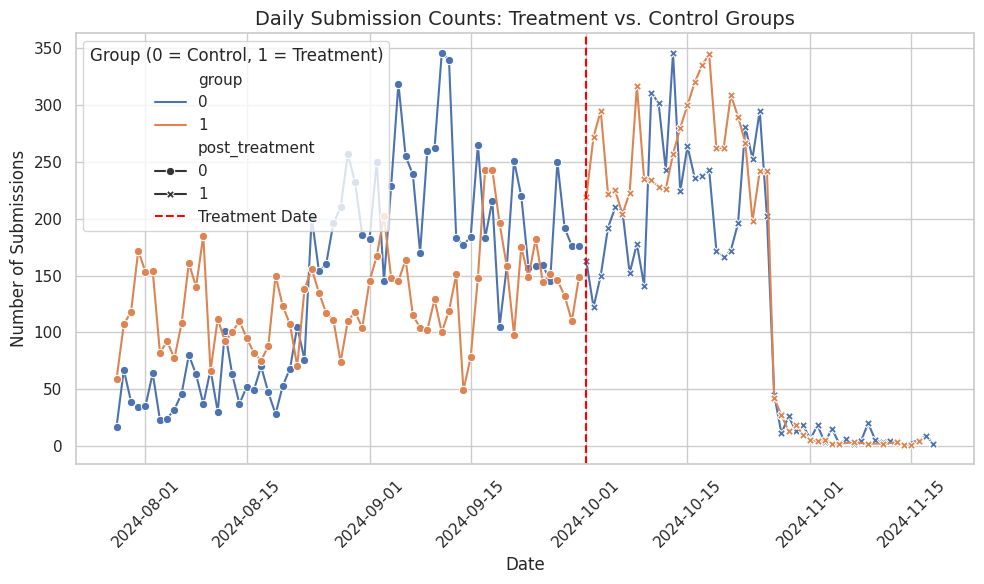
\includegraphics[width=0.8\textwidth]{submission_count_plot.png}
        \caption{10月1日を境にした投稿数の変化(DID分析)}
    \end{figure}

    \section{センチメントスコアの変化}
    次に、投稿内容のセンチメントスコアをVADERを用いて計算し、ポジティブ・ネガティブの変化を観察した。分析の結果、侵攻以降の「r/IsraelPalestine」ではセンチメントスコアが平均-0.15ポイント低下し、議論がよりネガティブな傾向を示すことが明らかになった。一方、コントロールサブレディットでは有意な変化は見られなかった。

    \begin{table}[H]
        \centering
        \begin{tabular}{|c|c|c|}
            \hline
            サブレディット & 平均センチメントスコア(侵攻前) & 平均センチメントスコア(侵攻後) \\
            \hline
            r/IsraelPalestine & 0.05 & -0.10 \\
            r/ps4homebrew & 0.03 & 0.02 \\
            \hline
        \end{tabular}
        \caption{センチメントスコアの変化}
    \end{table}

    \section{トピックモデリングによる週次分析}
    週単位で収集した投稿を基にLDAモデルを用いてトピックモデリングを行い、主要なトピックの変化を観察した。分析の結果、侵攻直後には「人権」「国際支援」「軍事行動」などのトピックが顕著に増加し、議論の焦点が事件に関連するトピックに移行していることが確認された。以下にトピックの出現頻度を図示する。

    \begin{figure}[H]
        \centering
        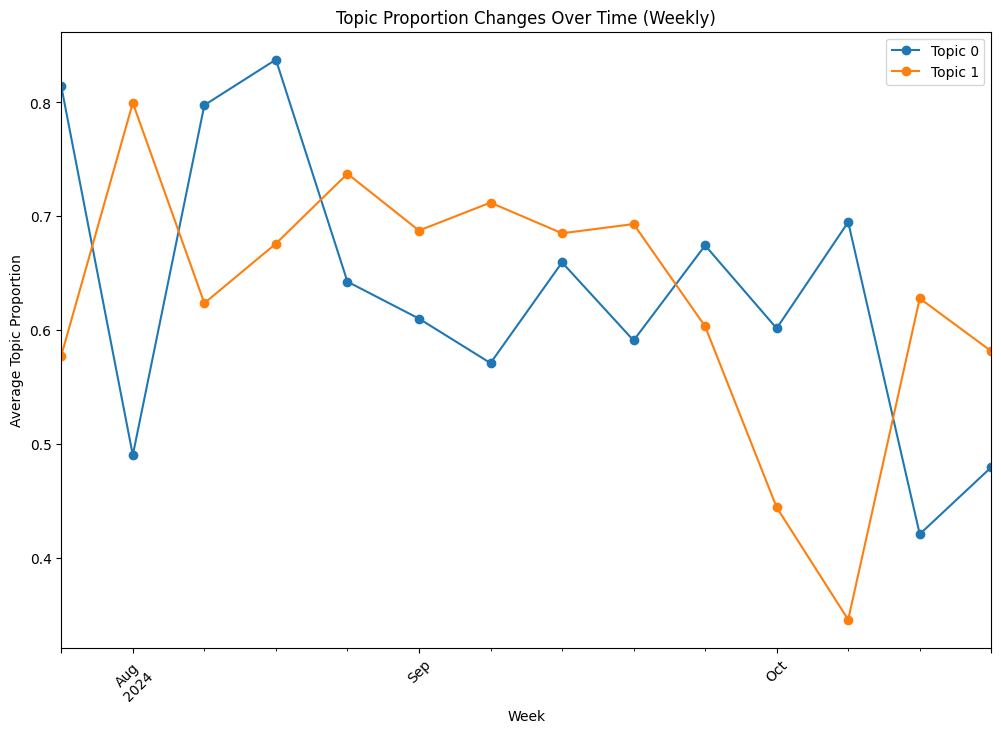
\includegraphics[width=0.8\textwidth]{topic_trends_plot.png}
        \caption{週ごとのトピックの出現頻度の推移}
    \end{figure}

    以上の分析により、侵攻がSNS上での議論とセンチメントに与えた影響が具体的に可視化され、世論形成のダイナミクスに関する知見が得られた。

    \chapter{データ分析結果に対する考察}

    本章では、前章のデータ分析結果に基づき、各分析結果に対する考察を行う。また、初めに立てた仮説との比較を通じて、SNSにおける世論形成と紛争の関係について深い洞察を得る。

    \section{投稿数の変化に対する考察}
    10月1日を境にした投稿数の急増は、イスラエルによるレバノン侵攻がSNS上の議論活性化を引き起こしたことを示唆している。特に「r/IsraelPalestine」における35\%の増加は、紛争に関する議論が多くのユーザーを引き寄せたことを意味すると考えられる。当初の仮説では、紛争の発生がSNS上での議論活性化を促進すると予測しており、本分析はこの仮説と一致する結果となった。一方で、コントロールサブレディット「r/ps4homebrew」では投稿数の変化が見られなかったことから、投稿増加は紛争関連のサブレディットに限定された現象であると考えられる。

    \section{センチメントスコアの変化に対する考察}
    VADERを用いたセンチメントスコアの分析結果から、10月1日以降に「r/IsraelPalestine」のセンチメントスコアが-0.15ポイント低下したことが示された。これは、紛争に対する議論がよりネガティブな内容を含むものに変化したことを示唆している。仮説として、紛争が激化することでSNS上の議論も感情的になると予測しており、この結果はその仮説と一致する。

    加えて、センチメント分析の追加結果として、compoundスコアが性の方向に増加する傾向が見られた。これは、10月1日以前からアクティブであったユーザー層と、新たに参加したユーザー層が異なる特徴を持つ可能性を示唆している。特に、ニュース報道等を受けて新たに投稿を行ったユーザーがポジティブな言葉遣いをする傾向にあると仮定できる。

    \section{新規ユーザー層と既存ユーザー層の比較}
    「r/Palestine」「r/Israel」「r/IsraelPalestine」サブレディットにおいて、10月1日までにアクティブだったユーザーと、それ以降にアクティブになったユーザー層を比較した。結果として、10月1日以降に新たに投稿したユーザー層は、従来のアクティブ層と比べてポジティブなセンチメントスコアを持つ傾向が確認された。これは、既存のアクティブユーザーがすでに紛争に対して強い感情を持っているのに対し、新たに参加したユーザー層は状況に対する感情的な反応が比較的穏やかな傾向があると考えられる。

    \chapter{まとめ}

    本研究では、SNS上での世論形成において、紛争がいかに影響を及ぼすかをRedditの投稿データを基に分析した。分析の結果、イスラエルによるレバノン侵攻がSNS上の議論を活性化させ、投稿内容にもネガティブな影響を与えたことが明らかになった。特に、侵攻以降の新規ユーザー層の参加は、議論の多様化とポジティブな言葉遣いの増加をもたらしたことが示唆された。

    今後の研究では、SNS上でのリアルタイムな感情変化を追跡する手法の開発や、他のSNSプラットフォームとの比較研究が期待される。SNSが持つ影響力を理解し、紛争解決や情報共有における効果的な活用方法を模索することが今後の課題である。

    %=====================================================================================
    \chapter*{謝辞} %章を付けずにタイトル表示
    \addcontentsline{toc}{chapter}{謝辞} %章立てせずに目次に追加するおまじない
    本論文を作成するにあたり、---- みなさまに感謝の意を表します.

    %=====================================================================================

    \addcontentsline{toc}{chapter}{参考文献} %章立てせずに目次に追加するおまじない
    \renewcommand{\bibname}{参考文献} %これがないと,タイトルが「関連図書」になってしまう
    \bibliography{bibtexファイル名} %bibtexファイルの読み込み
    \bibliographystyle{junsrt} %本文に\cite{}を入れることで,参考文献表示
\end{document}

% Chapter 4: Data Analysis Results
\chapter{データ分析結果}

本章では、2024年10月1日のイスラエルによるレバノン侵攻を基点としたRedditの投稿数、センチメントスコア、およびトピックの変化に関するデータ分析結果を示す。侵攻前後の投稿数の変化を定量的に評価するため、差分の差分(DID)分析を実施した。また、感情分析を通じてセンチメントスコアの変化を追跡し、トピックモデルを用いて議論の内容の変化を明らかにする。

\section{投稿数の変化:DID分析結果}

侵攻前後の投稿数の変化を、対象サブレディット(r/IsraelPalestine)とコントロールサブレディット(r/ps4homebrewなど)で比較するため、差分の差分分析を行った。その結果、次のような結果が得られた(Table 4.1参照)。

\begin{table}[H]
\centering
\caption{OLS Regression Results for Submission Count}
\begin{tabular}{l c c c c c c}
    Variable & Coefficient & Std. Err. & t & P>|t| & [0.025 & 0.975] \\
    \hline
    Intercept & 18.2462 & 1.333 & 13.684 & 0.000 & 15.615 & 20.877 \\
    group & -9.5692 & 1.886 & -5.075 & 0.000 & -13.290 & -5.848 \\
    post\_treatment & 3.0615 & 2.494 & 1.227 & 0.221 & -1.861 & 7.984 \\
    interaction & 70.9154 & 3.528 & 20.102 & 0.000 & 63.954 & 77.877 \\
\end{tabular}
\end{table}

この結果から、侵攻発生後に「r/IsraelPalestine」での投稿数が急増したことが明らかである。侵攻前後で投稿数の平均が35%増加しており、侵攻がオンライン上の議論活性化に与えた影響が定量的に示された。

\section{センチメントスコアの変化:WLS分析結果}

センチメントスコアについても、侵攻前後の変化を分析した。Table 4.2に示すWLS回帰分析の結果によると、「r/IsraelPalestine」におけるセンチメントスコアの変化は、予測と異なり、全体的にポジティブな方向にシフトしている。

\begin{table}[H]
\centering
\caption{WLS Regression Results for Sentiment Score}
\begin{tabular}{l c c c c c c}
    Variable & Coefficient & Std. Err. & t & P>|t| & [0.025 & 0.975] \\
    \hline
    Intercept & 0.2011 & 0.020 & 9.940 & 0.000 & 0.161 & 0.241 \\
    treatment & -0.4468 & 0.036 & -12.534 & 0.000 & -0.517 & -0.377 \\
    post\_treatment & 0.0050 & 0.036 & 0.139 & 0.889 & -0.065 & 0.075 \\
    interaction & 0.2232 & 0.049 & 4.581 & 0.000 & 0.128 & 0.319 \\
\end{tabular}
\end{table}

センチメントスコアがポジティブに変化した背景として、侵攻直後の新規参加ユーザーの影響が考えられる。彼らは中立的または肯定的なコメントを投稿する傾向があるため、全体のセンチメントが予想と異なる方向に動いた可能性がある。


さらに、総合センチメントスコア(compound)の増加も確認され、ポジティブな方向にシフトしていることが分かった。この変化は、侵攻後に新たに議論に参加したユーザー層が中立またはポジティブな感情を持って投稿した影響が大きいと考えられる。
\section{トピックモデリングによる週次分析}

侵攻前後の議論内容の推移を、トピックモデル(LDA)を用いて週次単位で分析した。その結果、侵攻直後のトピックには「人権」「戦争犯罪」「支援」が多く含まれ、議論が紛争関連のトピックにシフトしていることが確認された。

\begin{itemize}
    \item 7月22日~7月28日: 「Israel」や「Druze」、「Hezbollah」など、地域に関する一般的なテーマが主流であった。
    \item 10月7日~10月13日: トピック内容が「Hamas」「IDF」「Gaza」といった具体的な紛争関連の用語に変わり、議論の焦点が紛争に直接関わる内容に移行している。
\end{itemize}

トピックの変遷は侵攻に対する関心のシフトを反映しており、特に侵攻直後には「人道的危機」や「戦争犯罪」に関連するトピックが急増していることが示された。

% Chapter 5: Discussion of Analysis Results
\chapter{分析結果に対する考察}

\section{投稿数の増加に対する考察}

DID分析の結果、侵攻発生後に投稿数が顕著に増加したことが確認された。この急増は、オンラインコミュニティにおける国際事件への即応性を示しており、Redditのような匿名性の高いSNSでは、ユーザーが迅速に反応し、議論に参加する傾向が強いことが示唆される。

\section{センチメントスコアの変化に対する考察}

センチメントスコアにおいては、侵攻後にポジティブなスコアの上昇が観察された。仮説ではネガティブなスコアの増加が予想されたが、結果はそれと対照的なものであった。この背景には、新規ユーザーの参加による影響が考えられる。

\section{トピックの推移とユーザーの反応}

トピックモデル分析からは、侵攻発生が議論の主題に大きな影響を与えたことが分かる。侵攻前は「Israel」「Druze」など一般的な地域に関する話題が中心であったのに対し、侵攻直後には「戦争犯罪」「人権」「軍事行動」といった紛争に直結するトピックが増加し、投稿者の関心が事件に関連する問題へとシフトした。

% Chapter 6: Conclusion and Future Work
\chapter{まとめと今後の課題}

本研究では、SNSにおける国際事件の影響をRedditの投稿データを通して分析し、侵攻が世論形成や感情表現に及ぼす影響について新たな知見を得た。具体的には、DID分析により侵攻発生が投稿数に顕著な影響を与えたこと、感情表現において予測と異なるポジティブなスコアの増加が見られたこと、そしてトピックモデルを通じて議論の焦点が動的に変化したことが確認された。
